% Options for packages loaded elsewhere
\PassOptionsToPackage{unicode}{hyperref}
\PassOptionsToPackage{hyphens}{url}
\PassOptionsToPackage{dvipsnames,svgnames,x11names}{xcolor}
%
\documentclass[
  letterpaper,
  DIV=11,
  numbers=noendperiod]{scrartcl}

\usepackage{amsmath,amssymb}
\usepackage{lmodern}
\usepackage{iftex}
\ifPDFTeX
  \usepackage[T1]{fontenc}
  \usepackage[utf8]{inputenc}
  \usepackage{textcomp} % provide euro and other symbols
\else % if luatex or xetex
  \usepackage{unicode-math}
  \defaultfontfeatures{Scale=MatchLowercase}
  \defaultfontfeatures[\rmfamily]{Ligatures=TeX,Scale=1}
\fi
% Use upquote if available, for straight quotes in verbatim environments
\IfFileExists{upquote.sty}{\usepackage{upquote}}{}
\IfFileExists{microtype.sty}{% use microtype if available
  \usepackage[]{microtype}
  \UseMicrotypeSet[protrusion]{basicmath} % disable protrusion for tt fonts
}{}
\makeatletter
\@ifundefined{KOMAClassName}{% if non-KOMA class
  \IfFileExists{parskip.sty}{%
    \usepackage{parskip}
  }{% else
    \setlength{\parindent}{0pt}
    \setlength{\parskip}{6pt plus 2pt minus 1pt}}
}{% if KOMA class
  \KOMAoptions{parskip=half}}
\makeatother
\usepackage{xcolor}
\setlength{\emergencystretch}{3em} % prevent overfull lines
\setcounter{secnumdepth}{5}
% Make \paragraph and \subparagraph free-standing
\ifx\paragraph\undefined\else
  \let\oldparagraph\paragraph
  \renewcommand{\paragraph}[1]{\oldparagraph{#1}\mbox{}}
\fi
\ifx\subparagraph\undefined\else
  \let\oldsubparagraph\subparagraph
  \renewcommand{\subparagraph}[1]{\oldsubparagraph{#1}\mbox{}}
\fi

\usepackage{color}
\usepackage{fancyvrb}
\newcommand{\VerbBar}{|}
\newcommand{\VERB}{\Verb[commandchars=\\\{\}]}
\DefineVerbatimEnvironment{Highlighting}{Verbatim}{commandchars=\\\{\}}
% Add ',fontsize=\small' for more characters per line
\usepackage{framed}
\definecolor{shadecolor}{RGB}{241,243,245}
\newenvironment{Shaded}{\begin{snugshade}}{\end{snugshade}}
\newcommand{\AlertTok}[1]{\textcolor[rgb]{0.68,0.00,0.00}{#1}}
\newcommand{\AnnotationTok}[1]{\textcolor[rgb]{0.37,0.37,0.37}{#1}}
\newcommand{\AttributeTok}[1]{\textcolor[rgb]{0.40,0.45,0.13}{#1}}
\newcommand{\BaseNTok}[1]{\textcolor[rgb]{0.68,0.00,0.00}{#1}}
\newcommand{\BuiltInTok}[1]{\textcolor[rgb]{0.00,0.23,0.31}{#1}}
\newcommand{\CharTok}[1]{\textcolor[rgb]{0.13,0.47,0.30}{#1}}
\newcommand{\CommentTok}[1]{\textcolor[rgb]{0.37,0.37,0.37}{#1}}
\newcommand{\CommentVarTok}[1]{\textcolor[rgb]{0.37,0.37,0.37}{\textit{#1}}}
\newcommand{\ConstantTok}[1]{\textcolor[rgb]{0.56,0.35,0.01}{#1}}
\newcommand{\ControlFlowTok}[1]{\textcolor[rgb]{0.00,0.23,0.31}{#1}}
\newcommand{\DataTypeTok}[1]{\textcolor[rgb]{0.68,0.00,0.00}{#1}}
\newcommand{\DecValTok}[1]{\textcolor[rgb]{0.68,0.00,0.00}{#1}}
\newcommand{\DocumentationTok}[1]{\textcolor[rgb]{0.37,0.37,0.37}{\textit{#1}}}
\newcommand{\ErrorTok}[1]{\textcolor[rgb]{0.68,0.00,0.00}{#1}}
\newcommand{\ExtensionTok}[1]{\textcolor[rgb]{0.00,0.23,0.31}{#1}}
\newcommand{\FloatTok}[1]{\textcolor[rgb]{0.68,0.00,0.00}{#1}}
\newcommand{\FunctionTok}[1]{\textcolor[rgb]{0.28,0.35,0.67}{#1}}
\newcommand{\ImportTok}[1]{\textcolor[rgb]{0.00,0.46,0.62}{#1}}
\newcommand{\InformationTok}[1]{\textcolor[rgb]{0.37,0.37,0.37}{#1}}
\newcommand{\KeywordTok}[1]{\textcolor[rgb]{0.00,0.23,0.31}{#1}}
\newcommand{\NormalTok}[1]{\textcolor[rgb]{0.00,0.23,0.31}{#1}}
\newcommand{\OperatorTok}[1]{\textcolor[rgb]{0.37,0.37,0.37}{#1}}
\newcommand{\OtherTok}[1]{\textcolor[rgb]{0.00,0.23,0.31}{#1}}
\newcommand{\PreprocessorTok}[1]{\textcolor[rgb]{0.68,0.00,0.00}{#1}}
\newcommand{\RegionMarkerTok}[1]{\textcolor[rgb]{0.00,0.23,0.31}{#1}}
\newcommand{\SpecialCharTok}[1]{\textcolor[rgb]{0.37,0.37,0.37}{#1}}
\newcommand{\SpecialStringTok}[1]{\textcolor[rgb]{0.13,0.47,0.30}{#1}}
\newcommand{\StringTok}[1]{\textcolor[rgb]{0.13,0.47,0.30}{#1}}
\newcommand{\VariableTok}[1]{\textcolor[rgb]{0.07,0.07,0.07}{#1}}
\newcommand{\VerbatimStringTok}[1]{\textcolor[rgb]{0.13,0.47,0.30}{#1}}
\newcommand{\WarningTok}[1]{\textcolor[rgb]{0.37,0.37,0.37}{\textit{#1}}}

\providecommand{\tightlist}{%
  \setlength{\itemsep}{0pt}\setlength{\parskip}{0pt}}\usepackage{longtable,booktabs,array}
\usepackage{calc} % for calculating minipage widths
% Correct order of tables after \paragraph or \subparagraph
\usepackage{etoolbox}
\makeatletter
\patchcmd\longtable{\par}{\if@noskipsec\mbox{}\fi\par}{}{}
\makeatother
% Allow footnotes in longtable head/foot
\IfFileExists{footnotehyper.sty}{\usepackage{footnotehyper}}{\usepackage{footnote}}
\makesavenoteenv{longtable}
\usepackage{graphicx}
\makeatletter
\def\maxwidth{\ifdim\Gin@nat@width>\linewidth\linewidth\else\Gin@nat@width\fi}
\def\maxheight{\ifdim\Gin@nat@height>\textheight\textheight\else\Gin@nat@height\fi}
\makeatother
% Scale images if necessary, so that they will not overflow the page
% margins by default, and it is still possible to overwrite the defaults
% using explicit options in \includegraphics[width, height, ...]{}
\setkeys{Gin}{width=\maxwidth,height=\maxheight,keepaspectratio}
% Set default figure placement to htbp
\makeatletter
\def\fps@figure{htbp}
\makeatother
\newlength{\cslhangindent}
\setlength{\cslhangindent}{1.5em}
\newlength{\csllabelwidth}
\setlength{\csllabelwidth}{3em}
\newlength{\cslentryspacingunit} % times entry-spacing
\setlength{\cslentryspacingunit}{\parskip}
\newenvironment{CSLReferences}[2] % #1 hanging-ident, #2 entry spacing
 {% don't indent paragraphs
  \setlength{\parindent}{0pt}
  % turn on hanging indent if param 1 is 1
  \ifodd #1
  \let\oldpar\par
  \def\par{\hangindent=\cslhangindent\oldpar}
  \fi
  % set entry spacing
  \setlength{\parskip}{#2\cslentryspacingunit}
 }%
 {}
\usepackage{calc}
\newcommand{\CSLBlock}[1]{#1\hfill\break}
\newcommand{\CSLLeftMargin}[1]{\parbox[t]{\csllabelwidth}{#1}}
\newcommand{\CSLRightInline}[1]{\parbox[t]{\linewidth - \csllabelwidth}{#1}\break}
\newcommand{\CSLIndent}[1]{\hspace{\cslhangindent}#1}

\usepackage{fontspec}
\usepackage{multirow}
\usepackage{multicol}
\usepackage{colortbl}
\usepackage{hhline}
\newlength\Oldarrayrulewidth
\newlength\Oldtabcolsep
\usepackage{longtable}
\usepackage{array}
\usepackage{hyperref}
\usepackage{float}
\usepackage{wrapfig}
\KOMAoption{captions}{tableheading}
\makeatletter
\makeatother
\makeatletter
\makeatother
\makeatletter
\@ifpackageloaded{caption}{}{\usepackage{caption}}
\AtBeginDocument{%
\ifdefined\contentsname
  \renewcommand*\contentsname{Table of contents}
\else
  \newcommand\contentsname{Table of contents}
\fi
\ifdefined\listfigurename
  \renewcommand*\listfigurename{List of Figures}
\else
  \newcommand\listfigurename{List of Figures}
\fi
\ifdefined\listtablename
  \renewcommand*\listtablename{List of Tables}
\else
  \newcommand\listtablename{List of Tables}
\fi
\ifdefined\figurename
  \renewcommand*\figurename{Figure}
\else
  \newcommand\figurename{Figure}
\fi
\ifdefined\tablename
  \renewcommand*\tablename{Table}
\else
  \newcommand\tablename{Table}
\fi
}
\@ifpackageloaded{float}{}{\usepackage{float}}
\floatstyle{ruled}
\@ifundefined{c@chapter}{\newfloat{codelisting}{h}{lop}}{\newfloat{codelisting}{h}{lop}[chapter]}
\floatname{codelisting}{Listing}
\newcommand*\listoflistings{\listof{codelisting}{List of Listings}}
\makeatother
\makeatletter
\@ifpackageloaded{caption}{}{\usepackage{caption}}
\@ifpackageloaded{subcaption}{}{\usepackage{subcaption}}
\makeatother
\makeatletter
\@ifpackageloaded{tcolorbox}{}{\usepackage[many]{tcolorbox}}
\makeatother
\makeatletter
\@ifundefined{shadecolor}{\definecolor{shadecolor}{rgb}{.97, .97, .97}}
\makeatother
\makeatletter
\makeatother
\ifLuaTeX
  \usepackage{selnolig}  % disable illegal ligatures
\fi
\IfFileExists{bookmark.sty}{\usepackage{bookmark}}{\usepackage{hyperref}}
\IfFileExists{xurl.sty}{\usepackage{xurl}}{} % add URL line breaks if available
\urlstyle{same} % disable monospaced font for URLs
\hypersetup{
  pdftitle={The Mysterious Decline in Teen Suicidality in The US during the late 1990s},
  pdfauthor={Jin Di Lu},
  colorlinks=true,
  linkcolor={blue},
  filecolor={Maroon},
  citecolor={Blue},
  urlcolor={Blue},
  pdfcreator={LaTeX via pandoc}}

\title{The Mysterious Decline in Teen Suicidality in The US during the
late 1990s\thanks{Code and data are available at:
https://github.com/chrislu2234/suicidality\_report\_1990s}}
\usepackage{etoolbox}
\makeatletter
\providecommand{\subtitle}[1]{% add subtitle to \maketitle
  \apptocmd{\@title}{\par {\large #1 \par}}{}{}
}
\makeatother
\subtitle{A Statistical Analysis of the relationship between Legalized
Abortion and Teen Suicidality in late 1990s US.}
\author{Jin Di Lu}
\date{22 April 2023}

\begin{document}
\maketitle
\begin{abstract}
This study investigates the correlative relationship between abortion
rates and teen suicidality rates in the United States from 1973 to 2000.
Using annual time-series data on Abortions and Teen Suicide Rates, I
found a significant correlation between abortion rates and teen suicide
rates during the studied period, suggesting that the availability of
legal abortion might have contributed to the reduction in the number of
children born into adverse family conditions and, consequently,
alleviated the risk factors for teen suicidality. This research
highlights the importance of considering the broader social and
psychological implications of abortion policies and calls for further
exploration of the causal mechanisms and long-term impacts.
\end{abstract}
\ifdefined\Shaded\renewenvironment{Shaded}{\begin{tcolorbox}[sharp corners, borderline west={3pt}{0pt}{shadecolor}, boxrule=0pt, breakable, frame hidden, enhanced, interior hidden]}{\end{tcolorbox}}\fi

\hypertarget{introduction}{%
\section{Introduction}\label{introduction}}

The dramatic decline in teen suicide rates in the United States during
the the late 1990s and early 2000s is still considered a mystery in
present day in both public and academic discussion (Males, 1997). Like
the sudden decline in crime that also mysteriously occurred during the
late 1990s (Ford, 2016), teen suicide rates fell in the same fashion
following a similar trend. A wide array of factors may have contributed
to this phenomenon, and understanding these variables is crucial for
developing effective strategies to maintain and further improve mental
health among adolescents, especially during an where American teen
suicide rates are dramatically rising again (Rinehart and Barkley,
2023). In this paper, I will investigate the potential variables (in
this case, legalized abortion) and its correlative relationship with
teen suicidality in the United States. I will be focusing on the data
between 1973 and 2000, but also include data from up to 2016. By doing
so, I hope to shed light on the impact of the legalization of abortion
on the suicidality rates of young people, particularly in the context of
how it influences family functioning and relationships.

Several key studies and articles inform my research. Levitt and
Donohue's (\textbf{NBERw25863?}) seminal work, ``The Impact of Legalized
Abortion on Crime Over The Last Two Decades,'' attributes the enactment
of Roe v. Wade in 1973 as a major factor contributing to the decline in
crime rates across the nation. The authors argue that legalized abortion
allowed mothers in emotionally and economically challenging
circumstances to make informed choices they couldn't have before,
ultimately reducing the number of children born into adverse family
conditions to be incentivized towards criminal behavior.

Building on Levitt and Donohue's findings on the impact of legalized
abortion on adverse family conditions, in the qualitative study,
``Exploring the Family Factors Associated with Suicide Attempts among
Adolescents and Young Adults,''(\textbf{PMC8313455?}) establishes a
connection between the quality of family functioning and relationships
and the likelihood of teen suicidality. This connection provides a
potential pathway through which legalized abortion might have indirectly
contributed to the observed decline in teen suicidality during the
1990s.

Finally, ``The Relationship of Family Functioning and Suicidal Ideation
among Adolescents: The Mediating Role of Defeat and the Moderating Role
of Meaning in Life,'' (\textbf{PMC9740712?}) provide quantitative data
supporting the impact of family conditions on teen suicidality. Their
research further corroborates the findings of the previously mentioned
work and highlights the importance of considering family factors in
understanding the decline in teen suicide rates.

Drawing upon these studies and articles, I will conduct a comprehensive
analysis to examine the potential correlative relationship between
abortion rates and teen suicidality. My investigation will provide
valuable insights into the complex interplay between abortion policies,
family functioning, and suicidality among adolescents in the United
States.

In section 1 of this paper, I have introduced the significance of my
statistical question and the literature and discussion that surrounds
it. In section 2, I will expand on the dataset I have used for my
findings and describe the reasons why I have chosen certain variables
for my study. In section 3, I will describe the 4 models used to
investigate the correlation between abortion rates enabled by
legalization and teen suicide rates between the same time frame. I will
summarize my findings in section 4 and provide a discussion of them in
section 5 with acknowledgement of limitations and further actions that
can be taken to enhance this topic of research.

This paper uses R Core Team (2020), Wickham et al. (2019), and Wickham
(2016) to render, visualize, and clean all the data and graphs used in
the paper.

\hypertarget{sec-data}{%
\section{Data}\label{sec-data}}

For this study, I collected data on teen suicides and abortion rates
from two primary sources. The data on teen suicides were obtained from
the CDC WONDER's Compressed Mortality database, which encompasses
mortality and population counts for all U.S. counties. The CDC WONDER's
Compressed Mortality database is a comprehensive, public health
information system maintained by the Centers for Disease Control and
Prevention (CDC). It serves as a valuable resource for researchers,
public health professionals, and policymakers, providing access to a
wide range of data related to mortality and population counts for all
U.S. counties. The database enables users to retrieve and analyze vital
statistics data on various aspects of mortality, such as cause of death,
state, county, age, race, sex, and year.

The purpose of the Compressed Mortality database is to support
evidence-based decision-making and inform public health policies,
programs, and interventions. By providing a centralized and accessible
platform for mortality data, the CDC WONDER system helps users identify
trends, disparities, and patterns in mortality, which can be crucial for
understanding and addressing health-related issues. The database
typically serves to facilitate research and analysis on the health
status of the U.S. population, monitor changes in mortality over time,
and evaluate the effectiveness of public health initiatives. Moreover,
it assists in identifying areas that may require targeted interventions,
resources, or further investigation.

To collect data from the desired year ranges (1973-2016), I used three
different request forms: Mortality for 1999-2016 with ICD 10 codes,
Mortality for 1979-1998 with ICD 9 codes, and Mortality for 1968-1978
with ICD 8 codes. Each request form was submitted to obtain data on
suicide deaths among individuals aged 15-19 in the U.S. population,
including gender as a variable to identify any differences. The
definition of suicide remained consistent across all year ranges as
death caused by ``self-inflicted harm,'' despite varying ICD codes.
Further information on data retrieval can be found in the readme file.

The Guttmacher Institute's ``Pregnancies, Births and Abortions in the
United States'' report is a periodically updated publication that
provides comprehensive data on pregnancy outcomes, including abortions,
live births, and miscarriages, in the United States. The report presents
vital statistics on abortion rates, ratios, and numbers, as well as data
on pregnancy rates and birth rates among different age groups,
particularly focusing on women of reproductive age (15-49 years old).

The purpose of this report is to inform researchers, policymakers,
healthcare providers, and the general public about the current state of
reproductive health and pregnancy outcomes in the United States. By
maintaining and updating this report, the Guttmacher Institute
contributes to a better understanding of the factors that influence
reproductive health decisions and outcomes, as well as the effectiveness
of reproductive health policies and programs.

The Guttmacher Institutes' dataset is the same source used by Levitt and
Donohue to support their findings. I extracted information on abortion
rates between 1973 and 2017, where abortion rates are defined as the
number of abortions per 1,000 women in a given year. The dataset was
obtained by saving it as a CSV file from the Guttmacher Institute's
website. Additional details on data collection can be found in the
Methodology Appendix.

Both the CDC WONDER's Compressed Mortality database and the Guttmacher
Institute's Database and Research on Abortion Rates are comprehensive
and census-like in nature, minimizing the risk of biases in the data.
This robustness allows for a reliable analysis of the correlative
relationship between teen suicidality rates and abortion rates during
the studied period.

For the purposes of this paper, I collected both data up to 2016 from
CDC WONDER's Compressed Mortality Database and up to 2017 from
Guttmacher Institutes' abortion dataset. However, for parts of the
analysis, I will only analyze up to year 2000, as I believe the sudden
spike in teen suicide rates near the early 2010s is out of the scope of
this paper. I will be running a linear time-series regresesion to
explore how correlated the two factors may be, and whether or not
abortion rates can be a good explanation for the decline in teen
suicides in the late 1990s.

\hypertarget{models}{%
\section{Models}\label{models}}

\begin{Shaded}
\begin{Highlighting}[]
\CommentTok{\#Read CSVs}
\FunctionTok{setwd}\NormalTok{(}\StringTok{\textquotesingle{}C:/Users/chris/OneDrive/Documents/GitHub/suicidality\_report\_1990s\textquotesingle{}}\NormalTok{)}
\NormalTok{suicides }\OtherTok{\textless{}{-}} \FunctionTok{read\_csv}\NormalTok{(}\StringTok{"outputs/clean\_data/cleaned\_suicides.csv"}\NormalTok{)}
\end{Highlighting}
\end{Shaded}

\begin{verbatim}
Rows: 132 Columns: 6
-- Column specification --------------------------------------------------------
Delimiter: ","
chr (2): age group, gender
dbl (4): year, deaths, population, suicideratetotal

i Use `spec()` to retrieve the full column specification for this data.
i Specify the column types or set `show_col_types = FALSE` to quiet this message.
\end{verbatim}

\begin{Shaded}
\begin{Highlighting}[]
\NormalTok{abortions }\OtherTok{\textless{}{-}} \FunctionTok{read\_csv}\NormalTok{(}\StringTok{"outputs/clean\_data/cleaned\_abort.csv"}\NormalTok{)}
\end{Highlighting}
\end{Shaded}

\begin{verbatim}
Rows: 44 Columns: 6
-- Column specification --------------------------------------------------------
Delimiter: ","
dbl (6): year, abortionstotal, pregnanciestotal, population1544, abortionrat...

i Use `spec()` to retrieve the full column specification for this data.
i Specify the column types or set `show_col_types = FALSE` to quiet this message.
\end{verbatim}

Before engaging with the models, it is best to first understand the
data. In the exploratory stage of my analysis, I visually represented
teen suicide rates between 1973 to 2016. Afterwards, I explored the
differences in these rates between males and females, demonstrating to
what extent gender affects the statistics in teen suicides.

Next, I plotted abortion rates between the years 1973 to 2016. I then
plotted teen suicide rates against abortion rates as an attempt to
visually demonstrate the potential relationship between the two unimodal
plots. In modelling, I fit changes in abortion rates in relation to
changes in teen suicide rates to properly determine the extent of its
effects.

To engage in proper regression analysis, I also used O'Hara-Wild,
Hyndman, and Wang (2023), Wang, Cook, and Hyndman (2020), and Gohel and
Skintzos (2023). Fable offers a wide variety of packages dedicated to
forecasting models that use univariate and multivariate time series
forecasting models. For this paper, I used a time series linear
regression to explore the relationship and influences abortion rates may
have had on teen suicide rates. Tsibble was included to help transform
my dataframes into Time Series Tibbles that the time series linear
regression is able to use. Finally, I included patchwork to improve
presentation and overall clarity.

The Time series linear regression model I will be working with is
written below: \$\$

TSR\_\{t\} = \beta\emph{\{0\} + \beta}\{1\} AR\_\{t\}+ \epsilon\_\{t\}

\$\$ * The Dependent variable being investigated is Teen Suicide Rates,
denoted in TSR. * Beta0 represents the intercept, which is a point that
will be the starting point of the estimate. * Beta1 represents the
estimate (slope) of the regression, which represents the percent change
in TSR for increase in Abortion Rates (denoted as AR) * Epsilon
represents the innovation terms in a Time-Series Linear Model, such as
potential errors.

The first time series linear regression model looked at the relationship
between abortion rates and teen suicide rates between the years 1973 to
2000s without any adjustments made to either variables. The output was
very troubling, the coefficient reported an increase in suicides for
each percentage increase in abortions. This followed with a weak
R-squared, demonstrating that it was very difficult to explain suicide
rates in 1973-2000 with abortion rates in 1973-2000. This model's
inability to investigate the relationship between the two factors was
becase the time series linear regression model is unaware that natal
decisions will only have an impact on the population presented around
15-19 years later.

\$\$

TSR\_\{t\} = \beta\emph{\{0\} + \beta}\{1\} AAR\_\{t\}+ \epsilon\_\{t\}

\$\$ Hence, I produced a second model with an adjusted rate of abortion.
Rather than analyzing the relationship between suicide rates and
abortion strictly by their numbers in each of those years, I looked to
analyze the relationship between teen suicide rates and abortion rates
from 17 years prior. I believe this is the best way to represent the
impacts abortions have on the quality of life of children born after its
legalization in the United States.

In other words: * The Dependent variable being investigated is Teen
Suicide Rates, denoted in TSR. * Beta0 represents the intercept, which
is a point that will be the starting point of the estimate. * Beta1
represents the estimate (slope) of the regression, which represents the
percent change in TSR for increase in Adjusted Abortion Rates (denoted
as AR), AAR are 1973 abortion rates placed in 1990 as a way to represent
its effects. * Epsilon represents the innovation terms in a Time-Series
Linear Model, such as potential errors.

In this second model, I was able to demonstrate the relationship between
teen suicide rates and abortions, showing how an increase in abortions
from 17 years prior decreased teen suicides. Furthermore, the R Squared
of this model was a notable \textasciitilde0.500. I produced 2
additional models to see if this stands with male and female teens as
well. These two additional models are:

\$\$

TSRm\_\{t\} = \beta\emph{\{0\} + \beta}\{1\} AAR\_\{t\}+ \epsilon\_\{t\}

\[
\]

TSRf\_\{t\} = \beta\emph{\{0\} + \beta}\{1\} AAR\_\{t\}+ \epsilon\_\{t\}

\$\$ * The Dependent variable being investigated are Teen Suicide Rates
for males sand females, denoted in TSRm and TSRf. * Beta0 represents the
intercept, which is a point that will be the starting point of the
estimate. * Beta1 represents the estimate (slope) of the regression,
which represents the percent change in TSR for increase in Adjusted
Abortion Rates (denoted as AR), AAR are 1973 abortion rates placed in
1990 as a way to represent its effects. * Epsilon represents the
innovation terms in a Time-Series Linear Model, such as potential
errors.

Overall, I produced 6 figures and 4 models (which includes one table and
one figure each) to demonstrate the potential influences abortion rates
in 1973 may have had on teen suicide rates in the 1990s. By
demonstrating that the rise in abortion rates in 1973 can to a certain
extent statistically explain the decline in teen suicides in the 1990s,
I believe I have shown that there may be a significant relationship
between these two variables worthy of further investigation.

Figure 1: Teen Suicide Rates (Crude per 100 000) Total

\begin{verbatim}
Warning: Using `size` aesthetic for lines was deprecated in ggplot2 3.4.0.
i Please use `linewidth` instead.
\end{verbatim}

\begin{figure}

{\centering 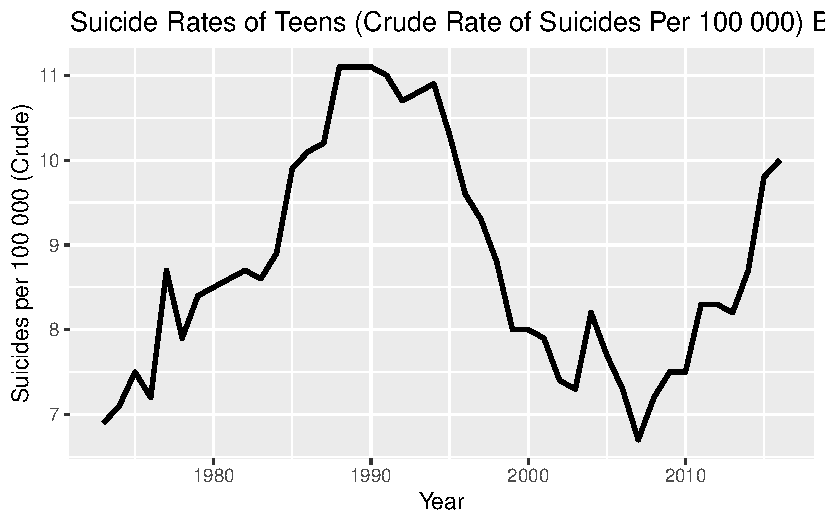
\includegraphics{paper_files/figure-pdf/fig-1-1.pdf}

}

\caption{\label{fig-1}Teen Suicide Rates (Crude per 100 000).}

\end{figure}

Figure~\ref{fig-1} represents the overall trend of crude teen suicide
rates per 100 000 (measured as deaths/population * 100 000) between the
years 1973 to 2016. If we look at the plot from before the 2000s, it
appears to be nearly unimodal. There is a rise that peaks around the
1990s, and immediately declines in 1995.

Figure 2: Teen Suicide Rates (Crude per 100 000) Male

\begin{figure}

{\centering 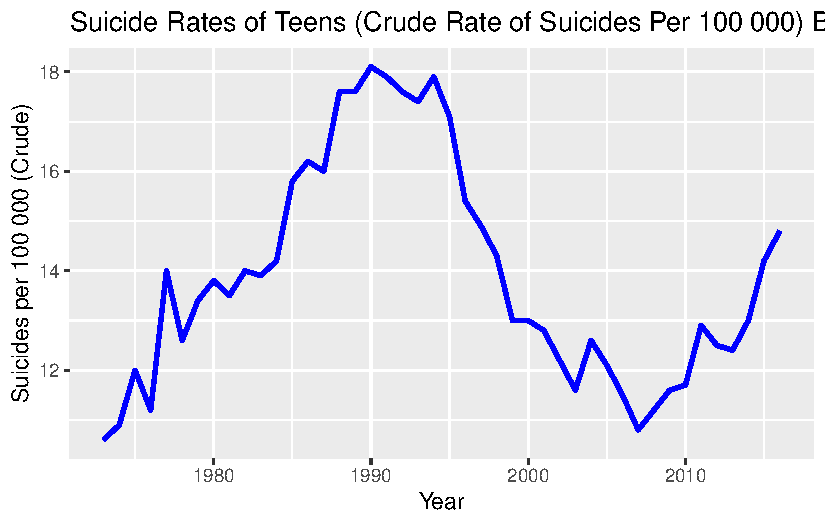
\includegraphics{paper_files/figure-pdf/fig-2-1.pdf}

}

\caption{\label{fig-2}Teen Suicide Rates (Crude per 100 000) for Males.}

\end{figure}

Figure~\ref{fig-2} represents crude male teen suicide rates per 100 000
between 1973 to 2016. Similar to Figure~\ref{fig-1}, this figure also is
nearly unimodal before the 2000s. There is a rise that peaks around the
1990s, and immediately declines in 1995. It is important to note here
that the rate of suicides amongst male teens is higher than that of the
total, indicating (as will be demonstrated by Figure~\ref{fig-3} later)
that female teen suicide rates are likely much lower.

Figure 3: Teen Suicide Rates (Crude per 100 000) Female

\begin{figure}

{\centering 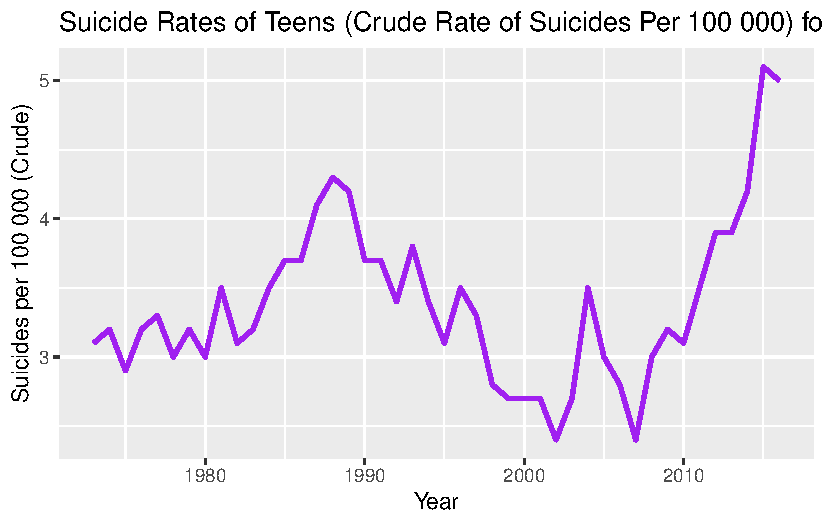
\includegraphics{paper_files/figure-pdf/fig-3-1.pdf}

}

\caption{\label{fig-3}Teen Suicide Rates (Crude per 100 000) for
Females.}

\end{figure}

Figure~\ref{fig-3} represents crude female teen suicide rates per 100
000 between 1973 to 2016. Contrary to male teen suicides, the
unimodality of this figure is not as severe.. Furthermore, the rate is
dramatically lower than that of male teens. Nevertheless, there is a
rise that peaks around the 1990s, and immediately declines in 1995.

Figure 4: Teen Suicide Rates (Crude per 100 000) Male, Female, Total.

\begin{figure}

{\centering 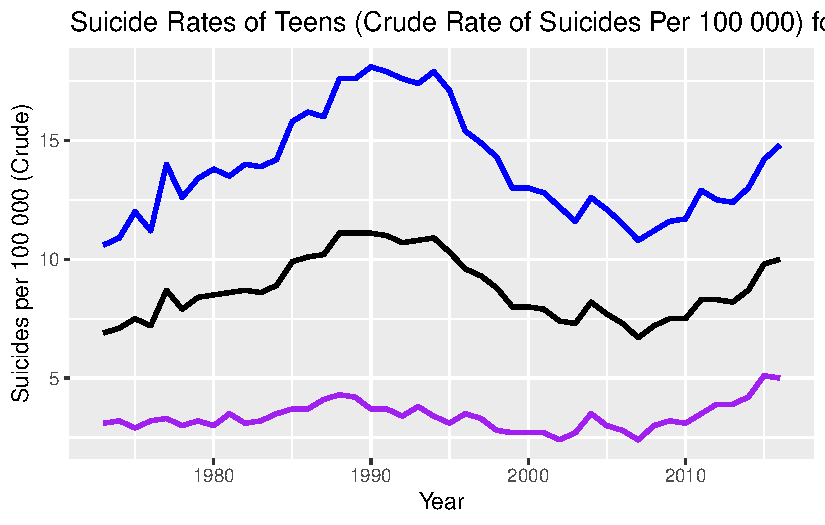
\includegraphics{paper_files/figure-pdf/fig-4-1.pdf}

}

\caption{\label{fig-4}Teen Suicide Rates (Crude per 100 000) for Males,
Females, and Averaged Total.}

\end{figure}

Figure~\ref{fig-4} represents crude male, female, and all teen suicide
rates per 100 000 between 1973 to 2016. As mentioned before, there is a
disproportionately high amount of male teen suicides in comparison to
females. this averages out in the black bar in the middle, which
represents the suicide rates of all teens overall.

Figure 5: Abortion Rates (Number of Abortions per 1 000 Women)

\begin{figure}

{\centering 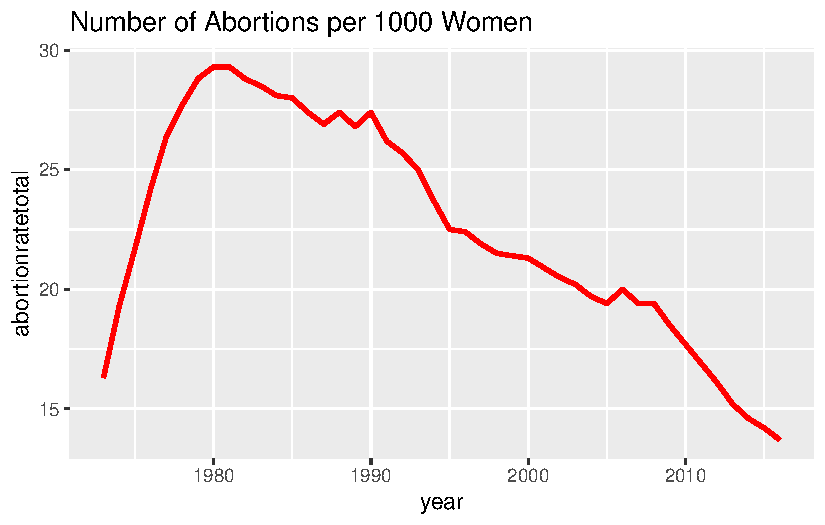
\includegraphics{paper_files/figure-pdf/fig-5-1.pdf}

}

\caption{\label{fig-5}Abortion Rates (Number of Abortions per 1 000
Women)}

\end{figure}

Figure~\ref{fig-5} represents abortion rates (Number of Abortions per
1000 Women) between 1973 to 2016. Red line follows the increase and
decreases of this trend over time. In this figure, we can see the sudden
rise in abortion rates after 1973 as a product of the Roe v. Wade
Supreme court Decision to Legalize Abortion. After this, we see how this
widespread legalization lead to an improvement to accessible abortion
resources and a spike in abortion rates. This trend peaks around the
1980s, and follows a slow decline afterwards.

Graph 6: Graph Teen Suicide Rates vs Abortion Rates

\begin{figure}

{\centering 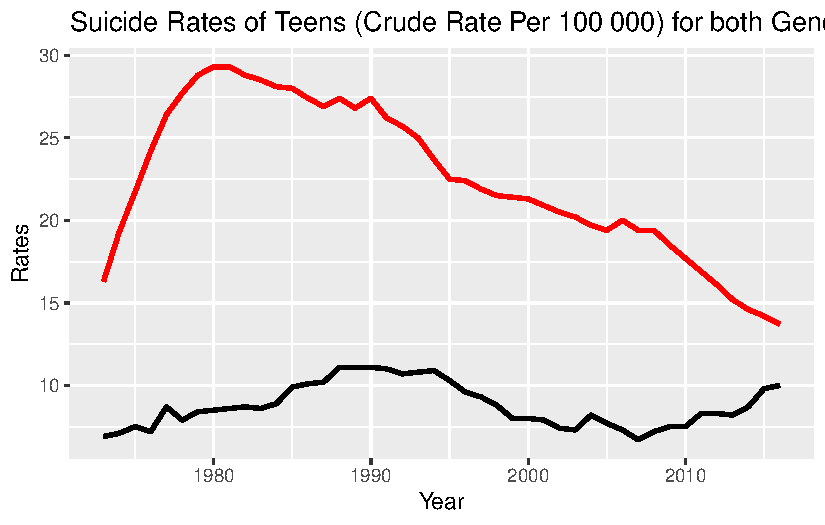
\includegraphics{paper_files/figure-pdf/fig-6-1.pdf}

}

\caption{\label{fig-6}Teen Suicide Rates vs.~Abortion Rates}

\end{figure}

Figure~\ref{fig-6} represents an attempt to plot teen suicide rates
against abortion rates. However, this plot provides very little
information on the topic, as the rates are not proportional to one and
another. But if we look closely, the dramatic increase in abortion rates
in 1973 can be argued to have manifested in the sharp declinee in teeen
suicides in 1995.

\hypertarget{results}{%
\section{Results}\label{results}}

Model 1: Teen Suicide Rates vs.~Abortion Rates

\begin{verbatim}
Series: suicideratetotal 
Model: TSLM 

Residuals:
    Min      1Q  Median      3Q     Max 
-1.8699 -1.1347 -0.2501  1.4252  1.9051 

Coefficients:
                  Estimate Std. Error t value Pr(>|t|)   
(Intercept)         5.4416     1.8209   2.988  0.00605 **
abortionratetotal   0.1499     0.0718   2.088  0.04672 * 
---
Signif. codes:  0 '***' 0.001 '**' 0.01 '*' 0.05 '.' 0.1 ' ' 1

Residual standard error: 1.273 on 26 degrees of freedom
Multiple R-squared: 0.1436, Adjusted R-squared: 0.1107
F-statistic: 4.361 on 1 and 26 DF, p-value: 0.04672
\end{verbatim}

\hypertarget{tbl-1}{}
\global\setlength{\Oldarrayrulewidth}{\arrayrulewidth}

\global\setlength{\Oldtabcolsep}{\tabcolsep}

\setlength{\tabcolsep}{0pt}

\renewcommand*{\arraystretch}{1.5}



\providecommand{\ascline}[3]{\noalign{\global\arrayrulewidth #1}\arrayrulecolor[HTML]{#2}\cline{#3}}

\begin{longtable}[c]{|p{0.75in}|p{0.75in}}

\caption{\label{tbl-1}Abortion Rates and its Effects on Teen Suicide Rates } \\ 


\ascline{1.5pt}{666666}{1-2}

\multicolumn{1}{>{\raggedright}m{\dimexpr 0.75in+0\tabcolsep}}{\textcolor[HTML]{000000}{\fontsize{11}{11}\selectfont{Terms}}} & \multicolumn{1}{>{\raggedleft}m{\dimexpr 0.75in+0\tabcolsep}}{\textcolor[HTML]{000000}{\fontsize{11}{11}\selectfont{Values}}} \\

\ascline{1.5pt}{666666}{1-2}\endhead



\multicolumn{1}{>{\raggedright}m{\dimexpr 0.75in+0\tabcolsep}}{\textcolor[HTML]{000000}{\fontsize{11}{11}\selectfont{Intercept}}} & \multicolumn{1}{>{\raggedleft}m{\dimexpr 0.75in+0\tabcolsep}}{\textcolor[HTML]{000000}{\fontsize{11}{11}\selectfont{5.442}}} \\





\multicolumn{1}{>{\raggedright}m{\dimexpr 0.75in+0\tabcolsep}}{\textcolor[HTML]{000000}{\fontsize{11}{11}\selectfont{AAR\ Coeff.}}} & \multicolumn{1}{>{\raggedleft}m{\dimexpr 0.75in+0\tabcolsep}}{\textcolor[HTML]{000000}{\fontsize{11}{11}\selectfont{-0.150}}} \\





\multicolumn{1}{>{\raggedright}m{\dimexpr 0.75in+0\tabcolsep}}{\textcolor[HTML]{000000}{\fontsize{11}{11}\selectfont{R2}}} & \multicolumn{1}{>{\raggedleft}m{\dimexpr 0.75in+0\tabcolsep}}{\textcolor[HTML]{000000}{\fontsize{11}{11}\selectfont{0.144}}} \\





\multicolumn{1}{>{\raggedright}m{\dimexpr 0.75in+0\tabcolsep}}{\textcolor[HTML]{000000}{\fontsize{11}{11}\selectfont{R2\ Adj}}} & \multicolumn{1}{>{\raggedleft}m{\dimexpr 0.75in+0\tabcolsep}}{\textcolor[HTML]{000000}{\fontsize{11}{11}\selectfont{0.568}}} \\





\multicolumn{1}{>{\raggedright}m{\dimexpr 0.75in+0\tabcolsep}}{\textcolor[HTML]{000000}{\fontsize{11}{11}\selectfont{P-Value}}} & \multicolumn{1}{>{\raggedleft}m{\dimexpr 0.75in+0\tabcolsep}}{\textcolor[HTML]{000000}{\fontsize{11}{11}\selectfont{0.047}}} \\

\ascline{1.5pt}{666666}{1-2}



\end{longtable}



\arrayrulecolor[HTML]{000000}

\global\setlength{\arrayrulewidth}{\Oldarrayrulewidth}

\global\setlength{\tabcolsep}{\Oldtabcolsep}

\renewcommand*{\arraystretch}{1}

\begin{figure}

{\centering 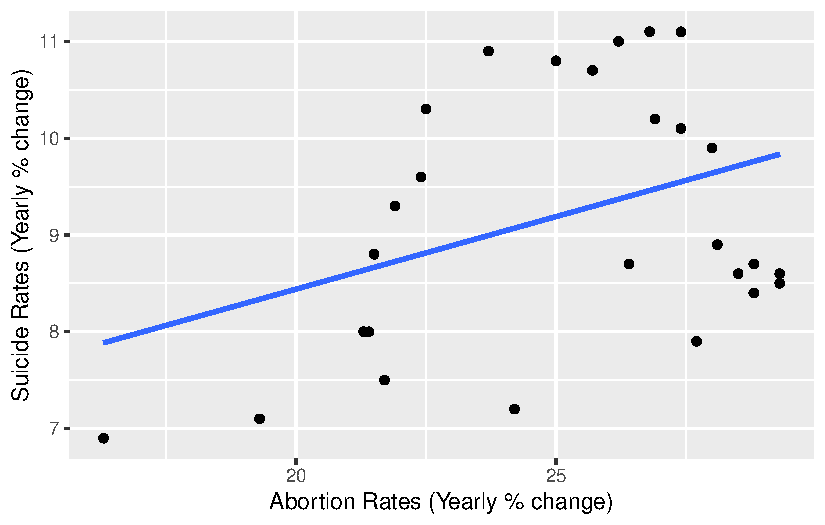
\includegraphics{paper_files/figure-pdf/fig-7-1.pdf}

}

\caption{\label{fig-7}Regression Line of Abortion Rates and its Effects
on Teen Suicide Rates}

\end{figure}

Summary Table~\ref{tbl-1} is the total summary output of the Time Series
Linear Regression in the time frame between 1973-2000. As mentioned
earlier, this output is concerning, as the coefficient suggests an
increase in suicides for increase in abortions. Additionally, the model
yields a weak R-squared (both multiple and adjusted), indicating that
this model is unable to explain suicide rates using abortion rates.

Figure~\ref{fig-7} plots changes in abortion rates with changes in
suicide rates. As mentioned above, this yields a regression model that
believes that the increase in abortion rates means an increase in
suicide rates.

As written earlier, the limitation of this model and both its table and
visual output is its inability to account for the fact that natal
decisions would only have impact on suicide rates approximately 15-19
years later. This inherent constraint in the model necessitated further
exploration of alternative approaches to better analyze the relationship
between these two variables effectively.

In Models 2, 3, and 4, I will implement a new variable: adjabtrates (for
Adjusted Abortion Rates) in my analysis to properly analyze the
relationship between abortion rates and teen suicide rates in the 1990s.
This new variable will simply place the value of abortion rates in 1973
with teen suicide rates in 1990s. In other words, I will use abortion
rates from 17 years prior to measure the suicide rates of teenagers. I
believe this is the best way to represent the impacts abortions have on
the quality of life of children born after its legalization in the
United States. In other words, I will use adjabtrates to properly
contextualize the decrease in teen suicides with the rise in abortion
rates.

Model 2: Teen Suicide Rates vs.~Adjusted Abortion Rates

\begin{verbatim}
Series: suicideratetotal 
Model: TSLM 

Residuals:
    Min      1Q  Median      3Q     Max 
-1.2775 -0.4344  0.1019  0.5341  1.2147 

Coefficients:
            Estimate Std. Error t value Pr(>|t|)    
(Intercept) 14.81223    1.52540    9.71 4.57e-06 ***
adjabtrates -0.19420    0.05902   -3.29  0.00937 ** 
---
Signif. codes:  0 '***' 0.001 '**' 0.01 '*' 0.05 '.' 0.1 ' ' 1

Residual standard error: 0.8441 on 9 degrees of freedom
Multiple R-squared: 0.546,  Adjusted R-squared: 0.4956
F-statistic: 10.83 on 1 and 9 DF, p-value: 0.0093746
\end{verbatim}

\hypertarget{tbl-2}{}
\global\setlength{\Oldarrayrulewidth}{\arrayrulewidth}

\global\setlength{\Oldtabcolsep}{\tabcolsep}

\setlength{\tabcolsep}{0pt}

\renewcommand*{\arraystretch}{1.5}



\providecommand{\ascline}[3]{\noalign{\global\arrayrulewidth #1}\arrayrulecolor[HTML]{#2}\cline{#3}}

\begin{longtable}[c]{|p{0.75in}|p{0.75in}}

\caption{\label{tbl-2}Adjusted Abortion Rates and its Effects on Teen Suicide Rates. } \\ 


\ascline{1.5pt}{666666}{1-2}

\multicolumn{1}{>{\raggedright}m{\dimexpr 0.75in+0\tabcolsep}}{\textcolor[HTML]{000000}{\fontsize{11}{11}\selectfont{Terms}}} & \multicolumn{1}{>{\raggedleft}m{\dimexpr 0.75in+0\tabcolsep}}{\textcolor[HTML]{000000}{\fontsize{11}{11}\selectfont{Values}}} \\

\ascline{1.5pt}{666666}{1-2}\endhead



\multicolumn{1}{>{\raggedright}m{\dimexpr 0.75in+0\tabcolsep}}{\textcolor[HTML]{000000}{\fontsize{11}{11}\selectfont{Intercept}}} & \multicolumn{1}{>{\raggedleft}m{\dimexpr 0.75in+0\tabcolsep}}{\textcolor[HTML]{000000}{\fontsize{11}{11}\selectfont{14.812}}} \\





\multicolumn{1}{>{\raggedright}m{\dimexpr 0.75in+0\tabcolsep}}{\textcolor[HTML]{000000}{\fontsize{11}{11}\selectfont{AAR\ Coeff.}}} & \multicolumn{1}{>{\raggedleft}m{\dimexpr 0.75in+0\tabcolsep}}{\textcolor[HTML]{000000}{\fontsize{11}{11}\selectfont{-0.194}}} \\





\multicolumn{1}{>{\raggedright}m{\dimexpr 0.75in+0\tabcolsep}}{\textcolor[HTML]{000000}{\fontsize{11}{11}\selectfont{R2}}} & \multicolumn{1}{>{\raggedleft}m{\dimexpr 0.75in+0\tabcolsep}}{\textcolor[HTML]{000000}{\fontsize{11}{11}\selectfont{0.546}}} \\





\multicolumn{1}{>{\raggedright}m{\dimexpr 0.75in+0\tabcolsep}}{\textcolor[HTML]{000000}{\fontsize{11}{11}\selectfont{R2\ Adj}}} & \multicolumn{1}{>{\raggedleft}m{\dimexpr 0.75in+0\tabcolsep}}{\textcolor[HTML]{000000}{\fontsize{11}{11}\selectfont{0.495}}} \\





\multicolumn{1}{>{\raggedright}m{\dimexpr 0.75in+0\tabcolsep}}{\textcolor[HTML]{000000}{\fontsize{11}{11}\selectfont{P-Value}}} & \multicolumn{1}{>{\raggedleft}m{\dimexpr 0.75in+0\tabcolsep}}{\textcolor[HTML]{000000}{\fontsize{11}{11}\selectfont{0.009}}} \\

\ascline{1.5pt}{666666}{1-2}



\end{longtable}



\arrayrulecolor[HTML]{000000}

\global\setlength{\arrayrulewidth}{\Oldarrayrulewidth}

\global\setlength{\tabcolsep}{\Oldtabcolsep}

\renewcommand*{\arraystretch}{1}

\begin{figure}

{\centering 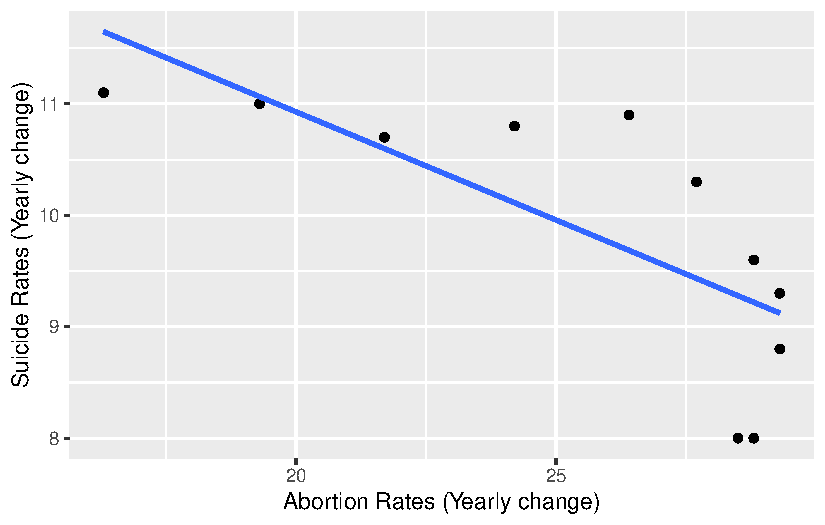
\includegraphics{paper_files/figure-pdf/fig-8-1.pdf}

}

\caption{\label{fig-8}Regression Line of Adjusted Abortion Rates and its
Effects on Teen Suicide Rates.}

\end{figure}

Summary Table~\ref{tbl-2} is the total summary output of the Time Series
Linear Regression in the time frame between 1990-2000. Instead of
analyzing the relationship between suicide rates and abortion rates
solely based on their values in the same year, I examined the
association between teen suicide rates and abortion rates from 17 years
prior in order to avoid the aforementioned limitation.

Figure~\ref{fig-8} beautifully depicts the analysis provided in
Table~\ref{tbl-2}, as the plot properly depicts the relationship between
abortion rates and suicide rates. As demonstrated in Figure~\ref{fig-8},
the peak in abortions from 17 years prior in abortion rates in 1973-1983
correlates with the decrease in suicide rates in 1990-2000.

I demonstrated a relationship between teen suicide rates and abortions,
revealing that an increase in abortions from 17 years prior was
associated with a decrease in teen suicides. The R-squared value for
this model was notably stronger, at approximately 0.500, indicating
better explanatory power. Furthermore the summary analysis also provides
a sensible estimate, demonstrating that an increase in abortion rates
meant on average a decrease in teen suicides.

Model 3: Teen Suicide Rates Male vs.~Abortion Rates

\begin{verbatim}
Series: suicideratetotal 
Model: TSLM 

Residuals:
     Min       1Q   Median       3Q      Max 
-2.07495 -0.72497  0.08471  0.67592  2.14347 

Coefficients:
            Estimate Std. Error t value Pr(>|t|)    
(Intercept) 24.32508    2.57289   9.454  5.7e-06 ***
adjabtrates -0.32457    0.09955  -3.260  0.00984 ** 
---
Signif. codes:  0 '***' 0.001 '**' 0.01 '*' 0.05 '.' 0.1 ' ' 1

Residual standard error: 1.424 on 9 degrees of freedom
Multiple R-squared: 0.5415, Adjusted R-squared: 0.4905
F-statistic: 10.63 on 1 and 9 DF, p-value: 0.0098359
\end{verbatim}

\hypertarget{tbl-3}{}
\global\setlength{\Oldarrayrulewidth}{\arrayrulewidth}

\global\setlength{\Oldtabcolsep}{\tabcolsep}

\setlength{\tabcolsep}{0pt}

\renewcommand*{\arraystretch}{1.5}



\providecommand{\ascline}[3]{\noalign{\global\arrayrulewidth #1}\arrayrulecolor[HTML]{#2}\cline{#3}}

\begin{longtable}[c]{|p{0.75in}|p{0.75in}}

\caption{\label{tbl-3}Adjusted Abortion Rates and its Effects on Male Teen Suicide Rates } \\ 


\ascline{1.5pt}{666666}{1-2}

\multicolumn{1}{>{\raggedright}m{\dimexpr 0.75in+0\tabcolsep}}{\textcolor[HTML]{000000}{\fontsize{11}{11}\selectfont{Terms}}} & \multicolumn{1}{>{\raggedleft}m{\dimexpr 0.75in+0\tabcolsep}}{\textcolor[HTML]{000000}{\fontsize{11}{11}\selectfont{Values}}} \\

\ascline{1.5pt}{666666}{1-2}\endhead



\multicolumn{1}{>{\raggedright}m{\dimexpr 0.75in+0\tabcolsep}}{\textcolor[HTML]{000000}{\fontsize{11}{11}\selectfont{Intercept}}} & \multicolumn{1}{>{\raggedleft}m{\dimexpr 0.75in+0\tabcolsep}}{\textcolor[HTML]{000000}{\fontsize{11}{11}\selectfont{24.325}}} \\





\multicolumn{1}{>{\raggedright}m{\dimexpr 0.75in+0\tabcolsep}}{\textcolor[HTML]{000000}{\fontsize{11}{11}\selectfont{AAR\ Coeff.}}} & \multicolumn{1}{>{\raggedleft}m{\dimexpr 0.75in+0\tabcolsep}}{\textcolor[HTML]{000000}{\fontsize{11}{11}\selectfont{-0.324}}} \\





\multicolumn{1}{>{\raggedright}m{\dimexpr 0.75in+0\tabcolsep}}{\textcolor[HTML]{000000}{\fontsize{11}{11}\selectfont{R2}}} & \multicolumn{1}{>{\raggedleft}m{\dimexpr 0.75in+0\tabcolsep}}{\textcolor[HTML]{000000}{\fontsize{11}{11}\selectfont{0.542}}} \\





\multicolumn{1}{>{\raggedright}m{\dimexpr 0.75in+0\tabcolsep}}{\textcolor[HTML]{000000}{\fontsize{11}{11}\selectfont{R2\ Adj}}} & \multicolumn{1}{>{\raggedleft}m{\dimexpr 0.75in+0\tabcolsep}}{\textcolor[HTML]{000000}{\fontsize{11}{11}\selectfont{0.491}}} \\





\multicolumn{1}{>{\raggedright}m{\dimexpr 0.75in+0\tabcolsep}}{\textcolor[HTML]{000000}{\fontsize{11}{11}\selectfont{P-Value}}} & \multicolumn{1}{>{\raggedleft}m{\dimexpr 0.75in+0\tabcolsep}}{\textcolor[HTML]{000000}{\fontsize{11}{11}\selectfont{0.010}}} \\

\ascline{1.5pt}{666666}{1-2}



\end{longtable}



\arrayrulecolor[HTML]{000000}

\global\setlength{\arrayrulewidth}{\Oldarrayrulewidth}

\global\setlength{\tabcolsep}{\Oldtabcolsep}

\renewcommand*{\arraystretch}{1}

\begin{figure}

{\centering 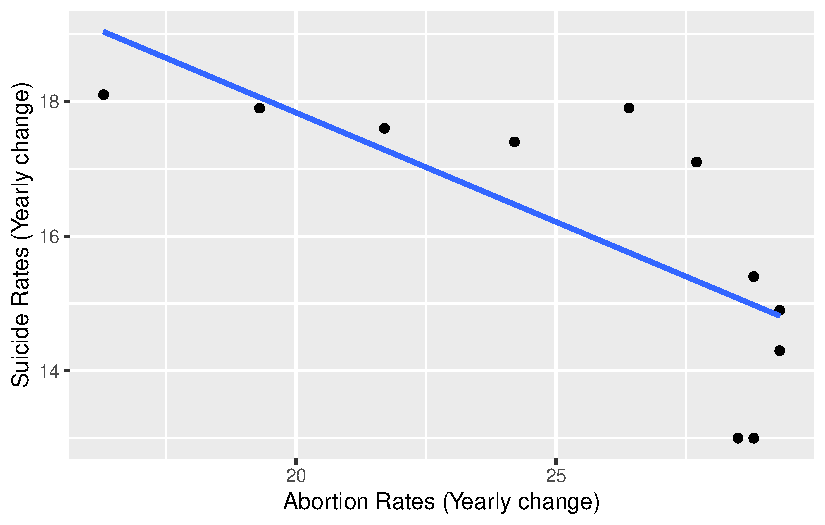
\includegraphics{paper_files/figure-pdf/fig-9-1.pdf}

}

\caption{\label{fig-9}Regression Line of Adjusted Abortion Rates and its
Effects on Male Teen Suicide Rates.}

\end{figure}

Summary Table~\ref{tbl-2} is the total summary output of the Time Series
Linear Regression in the time frame between 1990-2000 for male teen
suicide rates and adjusted abortion rates. Table~\ref{tbl-2} shows a
similar result to Table~\ref{tbl-1}, with a larger estimate.

Figure~\ref{fig-9} also corroborates with this analysis, as the plot
properly depicts the relationship between abortion rates and male teen
suicide rates. As demonstrated in Figure~\ref{fig-9}, the peak in
abortions from 17 years prior in abortion rates in 1973-1983 correlates
with the decrease in suicide rates in 1990-2000.

Overall, male teen suicide rates are significantly impacted by the rise
in abortion rates that occurred starting in 1973, indicating that
legalized abortion can have strong effects on the quality of life of
males during youth.

Model 4: Teen Suicide Rates Female vs.~Abortion Rates

\begin{verbatim}
Series: suicideratetotal 
Model: TSLM 

Residuals:
     Min       1Q   Median       3Q      Max 
-0.52897 -0.12779  0.01895  0.14707  0.54251 

Coefficients:
            Estimate Std. Error t value Pr(>|t|)    
(Intercept)  5.89038    0.60824   9.684 1.02e-06 ***
adjabtrates -0.09505    0.02322  -4.094  0.00178 ** 
---
Signif. codes:  0 '***' 0.001 '**' 0.01 '*' 0.05 '.' 0.1 ' ' 1

Residual standard error: 0.341 on 11 degrees of freedom
Multiple R-squared: 0.6037, Adjusted R-squared: 0.5677
F-statistic: 16.76 on 1 and 11 DF, p-value: 0.0017785
\end{verbatim}

\hypertarget{tbl-4}{}
\global\setlength{\Oldarrayrulewidth}{\arrayrulewidth}

\global\setlength{\Oldtabcolsep}{\tabcolsep}

\setlength{\tabcolsep}{0pt}

\renewcommand*{\arraystretch}{1.5}



\providecommand{\ascline}[3]{\noalign{\global\arrayrulewidth #1}\arrayrulecolor[HTML]{#2}\cline{#3}}

\begin{longtable}[c]{|p{0.75in}|p{0.75in}}

\caption{\label{tbl-4}Adjusted Abortion Rates and its Effects on Female Teen Suicide Rates } \\ 


\ascline{1.5pt}{666666}{1-2}

\multicolumn{1}{>{\raggedright}m{\dimexpr 0.75in+0\tabcolsep}}{\textcolor[HTML]{000000}{\fontsize{11}{11}\selectfont{Terms}}} & \multicolumn{1}{>{\raggedleft}m{\dimexpr 0.75in+0\tabcolsep}}{\textcolor[HTML]{000000}{\fontsize{11}{11}\selectfont{Values}}} \\

\ascline{1.5pt}{666666}{1-2}\endhead



\multicolumn{1}{>{\raggedright}m{\dimexpr 0.75in+0\tabcolsep}}{\textcolor[HTML]{000000}{\fontsize{11}{11}\selectfont{Intercept}}} & \multicolumn{1}{>{\raggedleft}m{\dimexpr 0.75in+0\tabcolsep}}{\textcolor[HTML]{000000}{\fontsize{11}{11}\selectfont{5.890}}} \\





\multicolumn{1}{>{\raggedright}m{\dimexpr 0.75in+0\tabcolsep}}{\textcolor[HTML]{000000}{\fontsize{11}{11}\selectfont{AAR\ Coeff.}}} & \multicolumn{1}{>{\raggedleft}m{\dimexpr 0.75in+0\tabcolsep}}{\textcolor[HTML]{000000}{\fontsize{11}{11}\selectfont{-0.095}}} \\





\multicolumn{1}{>{\raggedright}m{\dimexpr 0.75in+0\tabcolsep}}{\textcolor[HTML]{000000}{\fontsize{11}{11}\selectfont{R2}}} & \multicolumn{1}{>{\raggedleft}m{\dimexpr 0.75in+0\tabcolsep}}{\textcolor[HTML]{000000}{\fontsize{11}{11}\selectfont{0.604}}} \\





\multicolumn{1}{>{\raggedright}m{\dimexpr 0.75in+0\tabcolsep}}{\textcolor[HTML]{000000}{\fontsize{11}{11}\selectfont{R2\ Adj}}} & \multicolumn{1}{>{\raggedleft}m{\dimexpr 0.75in+0\tabcolsep}}{\textcolor[HTML]{000000}{\fontsize{11}{11}\selectfont{0.568}}} \\





\multicolumn{1}{>{\raggedright}m{\dimexpr 0.75in+0\tabcolsep}}{\textcolor[HTML]{000000}{\fontsize{11}{11}\selectfont{P-Value}}} & \multicolumn{1}{>{\raggedleft}m{\dimexpr 0.75in+0\tabcolsep}}{\textcolor[HTML]{000000}{\fontsize{11}{11}\selectfont{0.002}}} \\

\ascline{1.5pt}{666666}{1-2}



\end{longtable}



\arrayrulecolor[HTML]{000000}

\global\setlength{\arrayrulewidth}{\Oldarrayrulewidth}

\global\setlength{\tabcolsep}{\Oldtabcolsep}

\renewcommand*{\arraystretch}{1}

\begin{figure}

{\centering 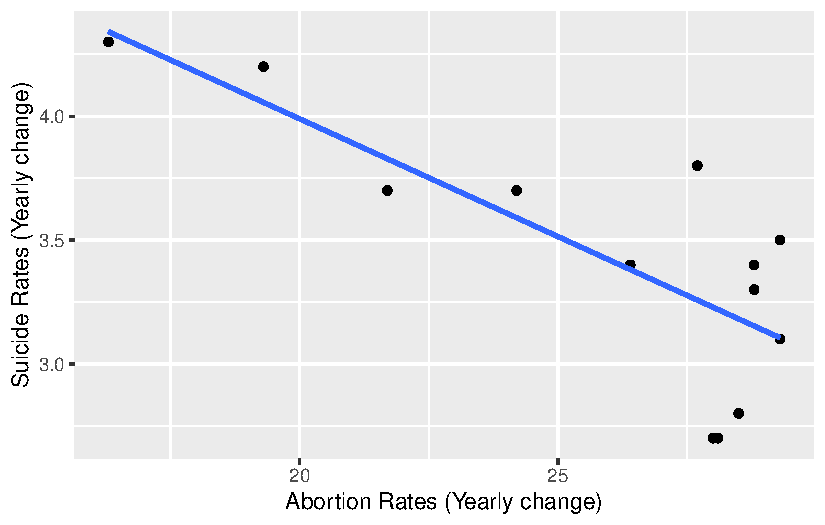
\includegraphics{paper_files/figure-pdf/fig-10-1.pdf}

}

\caption{\label{fig-10}Regression Line of Adjusted Abortion Rates and
its Effects on Female Teen Suicide Rates.}

\end{figure}

Summary Table~\ref{tbl-3} is the total summary output of the Time Series
Linear Regression in the time frame between 1990-2000 for female teen
suicide rates and adjusted abortion rates. Table~\ref{tbl-3} shows a
similar result to Table~\ref{tbl-2}, with a significantly smaller
estimate but much larger R-squared.This demonstrates that while the
impact of legalized abortion may affect female teen suicide rates to an
extent as great as it is on males, it is nevertheless worthy of
investigation.

Figure~\ref{fig-10} shows the relationship between abortion rates and
female teen suicide rates. As referred to in the comment on the larger
R-squared, the points fit the line much closely than the plots in
Figure~\ref{fig-9}

While female teen suicide rates are not as significantly impacted by the
rise in abortion rates as males, the strong fit nevertheless provides an
urge for further investigation. \# Discussion

\hypertarget{natal-policy-changes-only-manifest-18-years-after.}{%
\subsection{Natal Policy Changes Only Manifest 18 Years
After.}\label{natal-policy-changes-only-manifest-18-years-after.}}

The consequences of changes to natal laws become evident around 18 years
after they are implemented. This counter intuitive yet essential notion
suggests that present alterations to time-dependent events such as
changes to natal laws can result in significant, unpreventable
ramifications in the future and should demand an considerable amount of
attention beforehand.

To correctly evaluate the impact of abortion laws and changes
established 17 years prior on the suicide rates of 15-19 year-olds, I
had to transform the data by only analyzing suicide rates in 1990s with
abortion rates starting in 1973 rather than 1990s abortion rates. By
adjusting the data to account for the lag between the implementation of
natal laws and their outcomes, I was able to establish a more accurate
representation of the relationship between abortion rates and teen
suicide rates. This underscores the importance of ensuring that
variables are analyzed based on the appropriate time frame when their
outcomes manifest. It highlights the need for considering the temporal
nature of certain factors, as their effects do not always materialize
immediately. Not accounting for these temporal characteristics can
result in overlooking meaningful insights into the relationships between
variables and their potential consequences.

In light of the findings presented above, the recent Supreme Court
decision to overturn Roe v. Wade raises serious concerns regarding its
potential long-term consequences on public mental health. The connection
between abortion rates and teen suicide rates suggests that limited
access to safe and legal abortion services may result in a higher number
of children born into adverse family conditions. As past research has
shown, these challenging environments can significantly increase the
risk factors for teenage suicide. Eighteen years from now, we may
witness a considerable impact on the mental health of adolescents, as
they face will the consequences of restricted abortion access of today.
This potential fallout emphasizes the importance of comprehensive,
evidence-based natal policies that consider not only the immediate
implications of such decisions, but also their long-term effects on
population health and well-being.

\hypertarget{males-vs.-females}{%
\subsection{Males vs.~Females}\label{males-vs.-females}}

The analysis of teen suicide rates between 1973 and 2016 highlights
distinct differences in trends between teen males and females.
Figure~\ref{fig-2} and Figure~\ref{fig-3} reveal that male teen suicide
rates are considerably higher than female teen suicide rates. Both male
and female suicide rates experienced a rise that peaked in the 1990s and
subsequently declined in 1995. Interestingly, Table~\ref{tbl-2} and
Table~\ref{tbl-3} finds that changes in abortion rates have a more
substantial impact on male teen suicide rates compared to female teen
suicide rates.

As shown in Figure~\ref{fig-9} and Figure~\ref{fig-10}, the relationship
between abortion rates and teen suicide rates demonstrates a stronger
correlation for male teens. While the female teen suicide rates are
still affected to some extent, the influence of abortion rates is not as
pronounced as it is for males. This finding prompts further
investigation into the underlying reasons behind the differential impact
of abortion rates, evaluated as adverse family conditions, on male and
female teen suicide rates.

The observed disparities between male and female teen suicide rates in
relation to abortion rates emphasize the importance of understanding the
specific factors that contribute to these trends. A deeper exploration
of how and why adverse family conditions disproportionately affect male
teen suicides may shed light on targeted interventions and strategies
that can be employed to address this pressing public health issue.
Moreover, understanding the gender-specific dynamics at play can
contribute to more effective policies and programs aimed at reducing
teen suicidality and promoting mental health among adolescents.

\hypertarget{a-mystery-past-the-90s}{%
\subsection{A Mystery Past the 90s}\label{a-mystery-past-the-90s}}

While the primary focus of this research is on the relationship between
abortion rates and teen suicide rates between 1973 and 2000, it is
essential to acknowledge the alarming upsurge in teen suicide rates that
began in the 2010s. Although this recent increase falls outside the
scope of the current study, it represents a significant concern that
merits further investigation.

Considering that abortion rates served as a valuable indicator for teen
suicide rates in the past, the sharp rise in suicide rates during the
2010s might not be directly influenced by the growth of abortion
restrictions across many states in the US. In fact, abortion rates have
been on a consistent decline, while suicide rates have increased
dramatically. This apparent discrepancy suggests that other factors may
be contributing to the recent surge in teen suicide rates, which
requires additional research to identify and address the underlying
causes.

The recent Supreme Court decision to overturn Roe v. Wade could have
severe consequences 18 years down the line and may exacerbate the
already worrisome mental health crisis among teens. With the potential
for a growing number of children born into adverse family conditions due
to increased abortion restrictions, the long-term implications of this
policy change may significantly impact the mental health and well-being
of future generations. Consequently, it is crucial for researchers,
policymakers, and healthcare professionals to collaborate in
understanding and addressing the complex factors contributing to the
rise in teen suicide rates, and to develop evidence-based interventions
to mitigate the potential ramifications of recent policy changes on
adolescent mental health.

\hypertarget{weaknesses-and-next-steps}{%
\subsection{Weaknesses and Next Steps}\label{weaknesses-and-next-steps}}

This research, while providing valuable insights into the relationship
between abortion rates and teen suicide rates, has several limitations
that warrant further exploration. One of the primary weaknesses is the
lack of accounting for and controlling other variables that may impact
teen suicide rates. The current model focuses exclusively on the
association between abortion rates and suicidality, potentially
overlooking other influential factors that may contribute to changes in
teen suicide rates over time.

To improve the model, future research could consider incorporating
multiple variables that are believed to be significant in determining
teen suicidality. These additional factors may include socio-economic
status, access to mental health care, prevalence of substance abuse,
family dynamics, and the impact of social media on mental health. By
including these variables, we can develop a more comprehensive
understanding of the complex interplay of factors that contribute to
teen suicide rates, and identify specific areas for targeted
intervention and policy development.

Finally, the protection of reproductive rights is crucial not only for
upholding human well-being but also for preventing the potentially
disastrous consequences of future generations born into abhorrent family
conditions. As this study suggests, maintaining access to reproductive
healthcare and understanding the broader social and psychological
implications of reproductive policies are vital to ensuring the mental
health and well-being of adolescents. By prioritizing evidence-based
decision-making and collaboration between researchers, policymakers, and
healthcare professionals, society can work towards promoting the overall
health and welfare of all individuals, particularly our most vulnerable
populations.

\newpage

\appendix

\hypertarget{appendix}{%
\section*{Appendix}\label{appendix}}
\addcontentsline{toc}{section}{Appendix}

\hypertarget{additional-details}{%
\section{Additional details}\label{additional-details}}

\newpage

\hypertarget{references}{%
\section*{References}\label{references}}
\addcontentsline{toc}{section}{References}

\hypertarget{refs}{}
\begin{CSLReferences}{1}{0}
\leavevmode\vadjust pre{\hypertarget{ref-flextable}{}}%
Gohel, David, and Panagiotis Skintzos. 2023. \emph{Flextable: Functions
for Tabular Reporting}.
\url{https://CRAN.R-project.org/package=flextable}.

\leavevmode\vadjust pre{\hypertarget{ref-fable}{}}%
O'Hara-Wild, Mitchell, Rob Hyndman, and Earo Wang. 2023. \emph{Fable:
Forecasting Models for Tidy Time Series}.
\url{https://CRAN.R-project.org/package=fable}.

\leavevmode\vadjust pre{\hypertarget{ref-citeR}{}}%
R Core Team. 2020. \emph{R: A Language and Environment for Statistical
Computing}. Vienna, Austria: R Foundation for Statistical Computing.
\url{https://www.R-project.org/}.

\leavevmode\vadjust pre{\hypertarget{ref-tsibble}{}}%
Wang, Earo, Dianne Cook, and Rob J Hyndman. 2020. {``A New Tidy Data
Structure to Support Exploration and Modeling of Temporal Data.''}
\emph{Journal of Computational and Graphical Statistics} 29 (3):
466--78. \url{https://doi.org/10.1080/10618600.2019.1695624}.

\leavevmode\vadjust pre{\hypertarget{ref-ggplot2}{}}%
Wickham, Hadley. 2016. \emph{Ggplot2: Elegant Graphics for Data
Analysis}. Springer-Verlag New York.
\url{https://ggplot2.tidyverse.org}.

\leavevmode\vadjust pre{\hypertarget{ref-tidyverse}{}}%
Wickham, Hadley, Mara Averick, Jennifer Bryan, Winston Chang, Lucy
D'Agostino McGowan, Romain François, Garrett Grolemund, et al. 2019.
{``Welcome to the {tidyverse}.''} \emph{Journal of Open Source Software}
4 (43): 1686. \url{https://doi.org/10.21105/joss.01686}.

\end{CSLReferences}



\end{document}
